\begin{frame}
    \bigcenter{What is Scratch?}
\end{frame}

% \begin{frame}\frametitle{What is Scratch?}
%     \begin{figure}
%         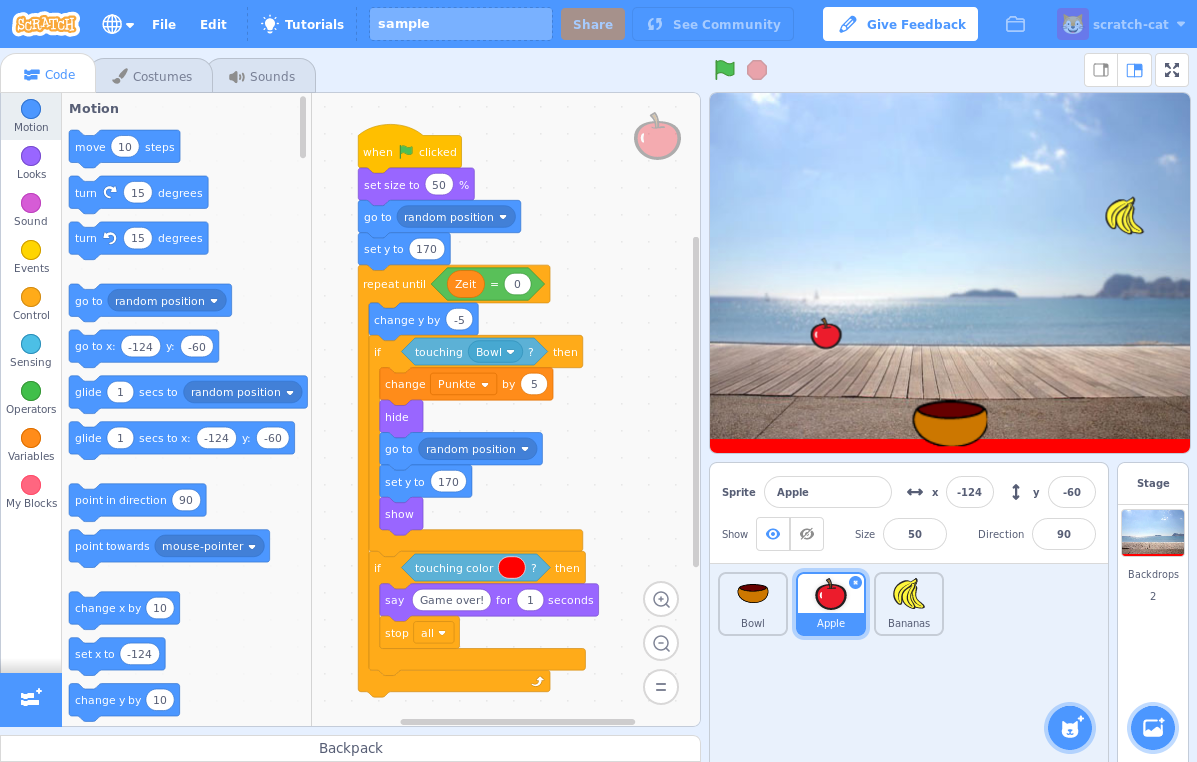
\includegraphics[width=.9\textwidth]{scratch-gui}
%         \caption{Scratch's GUI}
%     \end{figure}
% \end{frame}

\begin{frame}\frametitle{What is Scratch?}
    \begin{itemize}
        \item Block-based programming language
        \item Developed by the MIT media lab
        \item Programs create interactive animations on a stage
        \item Code is separated into scripts that are triggered by events
    \end{itemize}

    \pause

    \begin{figure}
        \centering
        \tikzset{>=latex,
                 arrow/.style={-{Latex[length=1.5mm, width=1.5mm]}},
                   box/.style={draw, text width=3.2cm, minimum height=0.7cm, text centered, rounded corners},
                 label/.style={text width=1.9cm}}

        \begin{tikzpicture}[scale=0.8, every node/.style={scale=0.8}]
            \node[box] at (0.0, 1.25) (step)   {Run active scripts in parallel};
            \node[box] at (0.0, 0.0) (render) {Render the stage};

            \node[label] at (-3.5, 0.75) {30 times per second};

            \draw[shorten >= 2pt, arrow, rounded corners]
                   (step)
                -- (render)
                -- ( 0.0, -1.0)
                -- (-2.4, -1.0)
                -- (-2.4,  2.5)
                -- ( 0.0,  2.5)
                -- (step);
        \end{tikzpicture}

        \caption{Scratch program execution}
    \end{figure}
\end{frame}

% Scratch 3.0 is accessed through a web interface
% Code is made up of blocks that are chosen from a drawer and sticked together
% These blocks include statements, expressions, variables, control structures, and also something called hats
% Hats are used to trigger scripts through a variety of different events
% For example the "green flag" event is the entry point of the program, and other events include clicks, key presses and messages from other scripts
% These scripts manipulate sprites on a stage to create animations
% Scratch Programs are usually very interactive, Scratch has blocks to use keyboard and mouse input, which often makes for game-like programs

\begin{frame}
    \bigcenter{Why automated testing for Scratch?}
\end{frame}

\begin{frame}\frametitle{Why automated testing for Scratch?}
    Many schools and universities deploy Scratch as a gentle introduction to programming.

    \pause
    \bigskip

    Grading Scratch assignments is very \textcolor{upfim}{time consuming}
    \begin{itemize}
        \item every project has to be opened individually
        \item programs require large amounts of \textcolor{upfim}{user interaction}
    \end{itemize}

    \pause
    \bigskip

    Some courses are attended by a \textcolor{upfim}{large number of students}
    \begin{itemize}
        \item manual testing for grading infeasible
        \item university of Utah: $> 200$~\cite{itch}
    \end{itemize}

    \pause
    \bigskip

    Additionally, students can use automated tests to get feedback for their own implementations.
\end{frame}
